\subsection{Methodology}

Our experiments are based on Social GAN by Agrim Gupta et al~\cite{Gupta_2018_CVPR}. It utilizes generative models to overcome the limitations of previous work. They build an LSTM-based encoder-decoder GAN capable of capturing the multimodality of trajectory prediction. In addition, they propose a novel pooling mechanism that enables the network to learn social norms among humans, and a $k$ variety loss that motivates the network to generate diverse samples.

In the following subsections, we will describe the key methods of our experiments.


\subsubsection{Generative Adversarial Networks}
\hfill \\
According to the research of Generative Adversarial Nets~\cite{gan}: a Generative Adversarial Network (GAN) consists of two network components, a discriminator $D$ and a generator $G$, which compete with each other. $G$ takes the input noise variable $z$ and generates the sample $G(z)$, $D$ takes the generated sample or training data as input $x$ and predicts the probability $D(x)$ that $x$ comes from the data and not generated by $G$. $D$ is trained to maximize the probability of assigning correct labels to training samples and generated samples, while $G$ is trained to minimize the correctness of $D$. In other words, $D$ and $G$ play a min-max game with the value function $V(G, D)$.
\begin{multline}
  \min_{G} \max_{D} V(G, D) = \mathbb{E}_{x \sim p_{\text{data}(x)}} \lbrack \log(D(x))\rbrack \\ + \mathbb{E}_{z \sim p_{z}(z)} \lbrack \log(1 - D(G(z))) \rbrack
\end{multline}

In our case, for pedestrian trajectory data, the generator is trained to generate possible future trajectories that have a distribution similar to the training data, given certain previously observed trajectories, while the discriminator learns to distinguish the rationality of the generated paths. These two networks are trained simultaneously. As the discriminators are learned, the generators are improved.

\subsubsection{InfoGAN}
\hfill \\
\begin{figure*}[ht]
  \centering
  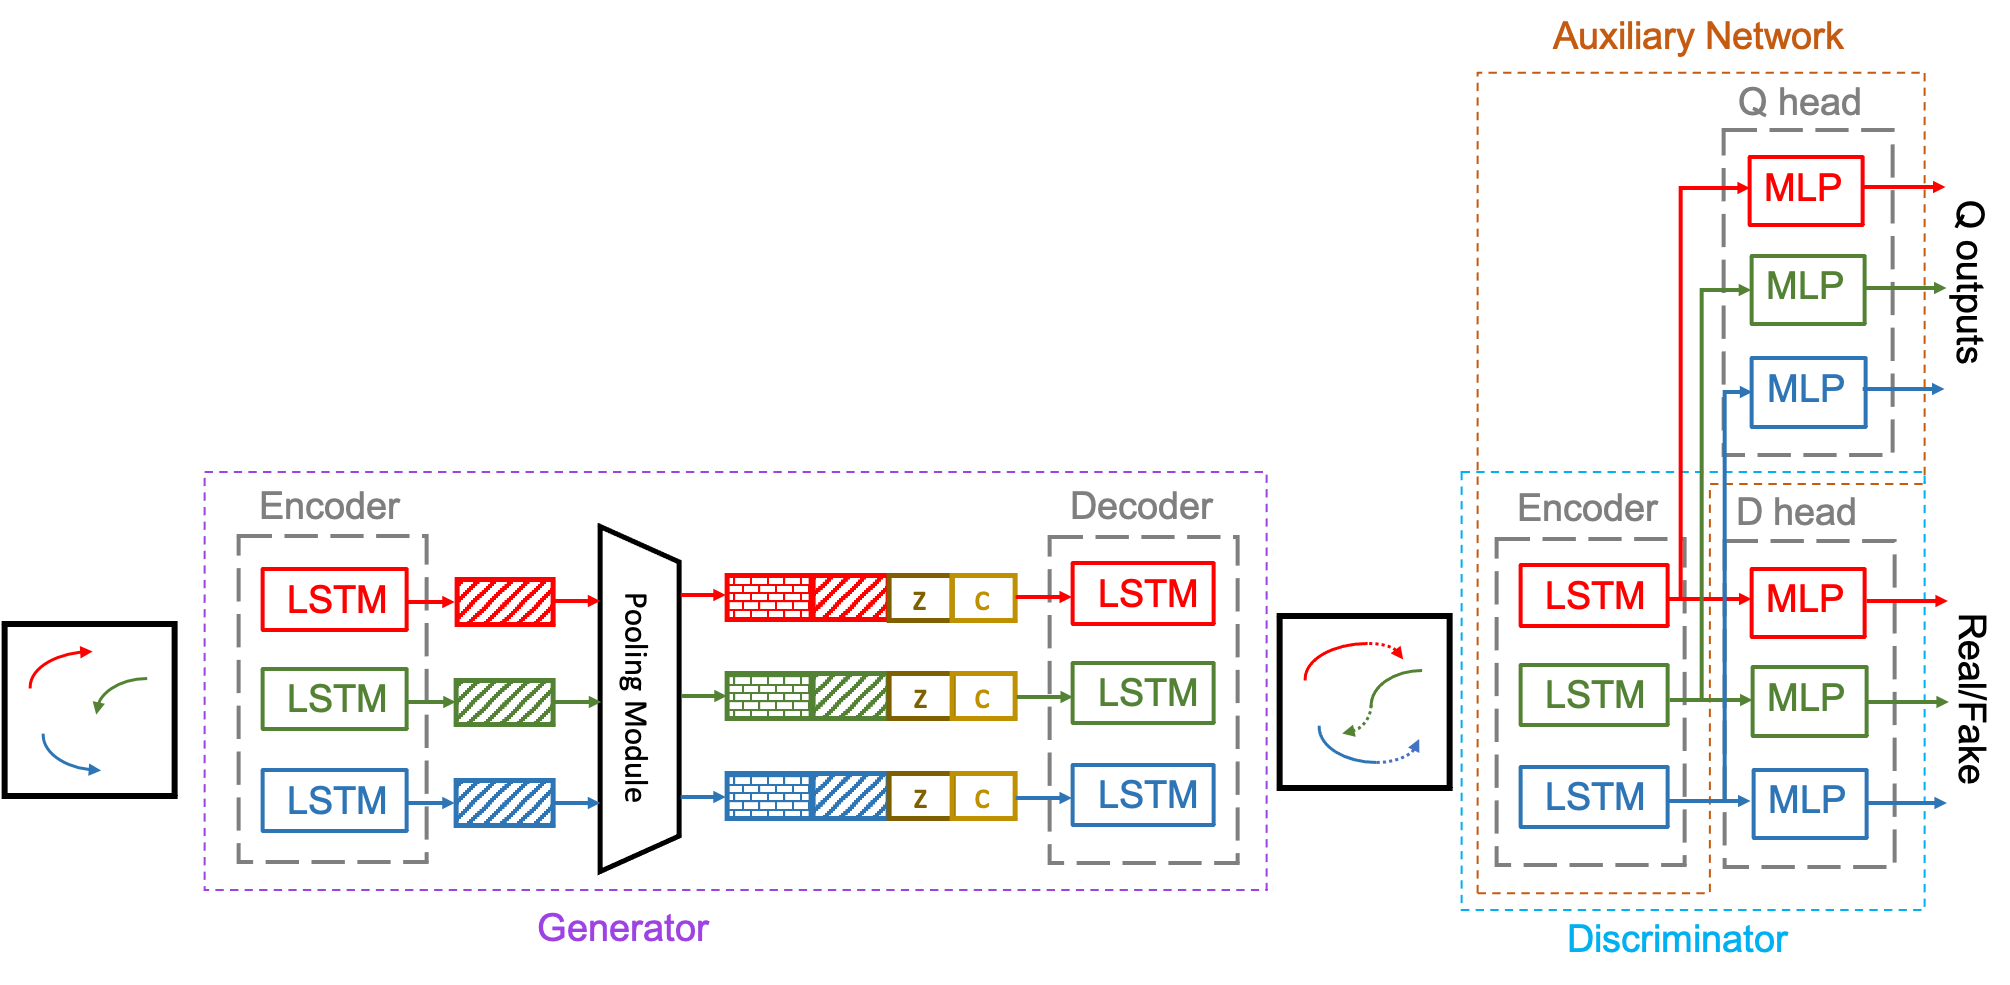
\includegraphics[width=0.8\textwidth]{figures/arch.png}
  \caption{Model Structure}{The latent code c is concated to the input of the generator decoder. The auxiliary network $Q$ is implemented in the way that $Q$ shared networks with $D$ and the head of $Q$ takes the extracted features from shared network as input.}
  \Description{model structure}
  \label{arch}
\end{figure*}
Information Maximizing Generative Adversarial Networks (InfoGAN) enable GANs to unsupervised learn disentangled representations by including information-theoretic regularization. It claims that the mutual information between a subset of the generator input (i.e., latent code $c$ decomposed from input $z$) and the generator output should be high. The lower bound of the mutual information $I(c; G(z, c))$ can be obtained as $$I(c; G(z, c)) \geq \mathbb{E}_{c \sim P(c), x \sim G(z, c)} \lbrack \log Q(c | x) \rbrack + H(c) \text{ , }$$ where only $Q(c | x)$ is an active variable and $x$ come from $G(z, c)$.

According to InfoGAN~\cite{infogan}, the additional work compared to GAN includes: $G$ takes the noise variable $z$ and the latent code $c$ as input to generate the sample $G(z, c)$. The additional auxiliary network $Q$ accepts the input $G(z, c)$ and outputs the parameters for $Q(c|G(z, c))$. G and Q are trained to maximize $Q(c | G(z, c))$. So, the min-max game is updated with a regularization: \[\min_{G,Q}\max_{D} \mathbf{V_{InfoGAN}}(D, G, Q) = \mathbf{V}(D, G) - \lambda I(c; G(z, c)) \]

In our work, we added parameterizable categorical latent codes and continuous latent codes to the generator, where the number of latent codes and the dimensionality of each categorical latent code are parameterizable. We implement the auxiliary network $Q$ in a way that it shares all network layers with $D$ except the last layer, and the final network of $Q$ is a multilayer perceptron that accepts the features extracted by the shared network $D_s$, and whose output depends on the distribution of the latent code. The implemented model is shown in Figure~\ref{arch}.

For the categorical latent code, we simply make it conform to the categorical distribution, so the output can be a softmax representation.
$$Q_{\text{head}}(D_s(G(z, c))) = MLP(D_s(G(z, c)); W_{Q}) = \hat c$$

For a continuous latent code, we make it conform to a Gaussian distribution, so the output can be Gaussian parameters, i.e., the expected value $\mu$ and the variance $\sigma^2$. For convenience, we implement the output as a logarithmic variance, so that the variance can be forced to be positive using an exponential transformation when calculating the loss.
$$Q_{\text{head}}(D_s(G(z, c))) = MLP(D_s(G(z, c)); W_{Q}) = [\: \mu \: \log(\sigma^2) \: ]$$
where $[\: \mu \: \log(\sigma^2) \: ]$ is the concatenation of $\mu$ and $\log(\sigma^2)$.

\subsubsection{Loss}
\hfill \\
Our experiments attempt to disentangle the latent code so that the latent code can correspond to the semantic features of the data. To enrich our expression, we allow two types of latent codes, categorical latent codes and continuous latent codes. These two types of simple latent codes can cover most of the controllable factors. On the basis of that, we can introduce a series of semantic factors. For example, velocity and direction can be represented as continuous latent codes and scenes can be expressed as categorical latent codes.

For categorical latent code $c$ (which conforms to the categorical distribution), we can use cross entropy as a loss function to maximize the information between the code $c$ and the trajectory generated by code $c$.
$$\mathcal{L}_{\text{disc}} (c, Q(G(z, c))) = CE(c, Q(G(z, c))) $$

For a continuous latent code $c$ (which conforms to a Gaussian distribution), we can use the negative log likelihood loss to maximize the information between the code $c$ and the trajectory generated by code $c$.
$$\mathcal{L}_{\text{cont}} (c, Q(G(z, c))) = NLL(c, Q(G(z, c))) $$

The categorical latent code loss and the continuous latent code loss can be scaled by the hyperparameters $\lambda_{disc}$ and $\lambda_{cont}$, respectively.

\subsubsection{Regularization}
\hfill \\
To constrain the independence of each code, we added a regularization. We claim that the variation of generated sample contributed by one code should be orthogonal with the variation contributed by code another code. That is, for $c_1, c_2$, we have:
  $$ (\frac {G(c_1 + \delta, c_2) - G(c_1, c_2, c_3)} {\delta})^T (\frac {G(c_1, c_2 + \delta, c_3) - G(c_1, c_2)} {\delta}) = 0$$
We use the encoder in generator to get the embedding of the trajectory and claim that the variation between embeddings should be orthogonal.

\subsection{Experimental Setup}
The first goal of our experiments is not to worsen the performance of the original SocialGAN network. Because we just added some latent codes to the original network, we did not reduce the dimensionality of the noise vectors or make any other changes. The second goal is to disentangle some factors with our implementation of InfoGAN, which is also the main goal of our experiments. To achieve these goals, we introduced the following metrics, baselines, and measures of the disentanglement.

\subsubsection{Evaluation Metrics}
\hfill \\
We evaluate our work with the following metrics that have been used extensively in previous work~\cite{Gupta_2018_CVPR, distant_prediction, Alahi16}.

\textbf{Average Displacement Error (ADE)}:  Average Euclidean distance between ground truth and the prediction over all predicted time steps.
$$\text{ADE}_{T} = \frac 1 T \sum_{t=0}^{T} \lVert \langle x^t, y^t \rangle - \langle \hat x^t, \hat y^t \rangle \lVert_{2} \text{ . }$$

\textbf{Final Displacement Error (FDE)}: Euclidean distance between ground truth and the prediction at the final time step.
$$\text{FDE}_{T} = \lVert \langle x^T, y^T \rangle - \langle \hat x^T, \hat y^T \rangle \lVert_{2} \text{ . }$$

Consistent with Social GAN~\cite{Gupta_2018_CVPR}, we performed experiments with $T$ equal to $8$ or $12$, which is also a common choice.


\subsubsection{Baselines}
\hfill \\
Since our experiments are based on Social GAN, we directly choose Social GAN as our baseline for comparison. We followed the same strategy as Social GAN, using the leave-on-out method for training (training on 4 sets and testing on the remaining sets). In particular,  we can set some parameters regarding Social GAN. We can train a model containing social pooling net, using k variety loss. Then in testing, we generate $N$ samples for the next $T$ steps trajectory and report the minimum ADE and FDE in these $N$ samples. In our experiments, we chose two specific settings of Social GAN as the baseline:
\begin{itemize}
  \item SGAN-20VP-20 (training Social GAN with social pooling module using 20 variety loss, and generating 20 samples in testing)
  \item SGAN-20V-20 (training Social GAN using 20 variety loss, and generating 20 samples in testing)
\end{itemize}

\subsubsection{Disentanglement Measuring}
\hfill \\
To measure the disentanglement of our implementation of InfoGAN, we utilized latent traversal. We generate traversals in this way: we first randomly select $N$ trajectories. For each of these trajectories, we traverse over a single latent code while keep other units fixed, and then we generate trajectory for each traversal value of this latent code with the corresponding inputs (noise, other codes and this traversed code) and plot them. Then we obtain the traversals of a single latent code over $N$ samples.

\begin{itemize}
  \item For categorical latent codes with $d$ categories, the traversal is over $d$ categorical latent variables representing each category.
  \item For a continuous latent code, the traversal is over range $(-2, 2)$. We perform linear interpolation to get 10 points between $(-2, 2)$, which can be the common values of the latent code that conforms to distribution $\mathcal{N}(0, 1)$.
\end{itemize}

We inspect the latent traversal for $N$ samples. We expect to find some common patterns of variations in a single latent codes, which means that the code is disentangled and encode with semantic meaning.